%
% This presentation is for use at the MDACC Medical Physics Trainee 2015 Summer
% Seminar Series on July 6, 2015.
%

\documentclass{beamer}
\usepackage{amsmath}
\usepackage{graphicx}
\usetheme{Warsaw}
\graphicspath{{Images/}}

%%%%%%%%%%%%%%%%%%%%%%%%%%%%%%%%%%%%%%%%%%%%%%%%%%%%%%%%%%%%%%%%%%%%%%%%%%%
% Title Page
%%%%%%%%%%%%%%%%%%%%%%%%%%%%%%%%%%%%%%%%%%%%%%%%%%%%%%%%%%%%%%%%%%%%%%%%%%%
\title[Spinal Cord DWI with ss-EPI]{DWI of the Spinal Cord with Reduced FOV Single-Shot EPI}
\author{Drew Mitchell}
\institute{MD Anderson Cancer Center}
\date{June 17, 2015}
%\AtBeginSection[]
%{{
%\setbeamertemplate{headline}{}
%\frame{\tableofcontents[currentsection]}
%}}

\begin{document} 
{
\setbeamertemplate{headline}{}
\frame{\titlepage}
\begin{frame}{Table of Contents}
\tableofcontents
\end{frame}
}

%%%%%%%%%%%%%%%%%%%%%%%%%%%%%%%%%%%%%%%%%%%%%%%%%%%%%%%%%%%%%%%%%%%%%%%%%%%
% Introduction
%%%%%%%%%%%%%%%%%%%%%%%%%%%%%%%%%%%%%%%%%%%%%%%%%%%%%%%%%%%%%%%%%%%%%%%%%%%
\section{Introduction}

\begin{frame}{Introduction}
\begin{itemize}
	\item Spinal cord diffusion-weighted imaging (DWI) can diagnose disorders from fiber tract damage
	\item Several challenges:
	\begin{itemize}
		\item Magnetic field inhomogeneities around spine create off-resonance artifacts
		\item Partial volume effects from CSF and lipid
		\item Spinal cord cross section very small
		\item Bulk physiologic motion from heart, breathing, swallowing, CSF pulsation
	\end{itemize}
	\item Result is low-signal, low-resolution DW images with artifacts in spinal cord
\end{itemize}
\end{frame}

\begin{frame}{Introduction}
\begin{itemize}
	\item Single-shot echo planar imaging (ss-EPI) most frequently used technique for DWI
	\begin {itemize}
		\item Acquires whole k-space after single excitation pulse
		\item No ghosting artifacts from motion-induced phase errors
	\end {itemize}
	\item Long readout experiences $T_2^*$ decay
\end{itemize}
\end{frame}

\begin{frame}{Introduction}
\begin{itemize}
	\item Spinal cord imaging benefits from reduced FOV applications
	\item Reduced FOV methods decrease the readout duration and reduce off-resonance artifacts
	\item Excited FOV in PE direction reduced by 2D spatially selective echo-planar RF excitation pulse and $180^{\circ}$ refocusing RF pulse
	\item Allows multi slice imaging and suppresses fat signal
\end{itemize}
\end{frame}
	
%%%%%%%%%%%%%%%%%%%%%%%%%%%%%%%%%%%%%%%%%%%%%%%%%%%%%%%%%%%%%%%%%%%%%%%%%%%
% Theory
%%%%%%%%%%%%%%%%%%%%%%%%%%%%%%%%%%%%%%%%%%%%%%%%%%%%%%%%%%%%%%%%%%%%%%%%%%%
\section{Theory}

\begin{frame}{Theory}
\begin{columns}[T]
	\begin{column}[T]{5cm}
		Standard DW spin-echo ss-EPI sequence, with excitation pulse replaced with $90^{\circ}$ 2D spatially selective echo-planar RF pulse
	\end{column}
	\begin{column}[T]{5cm}
		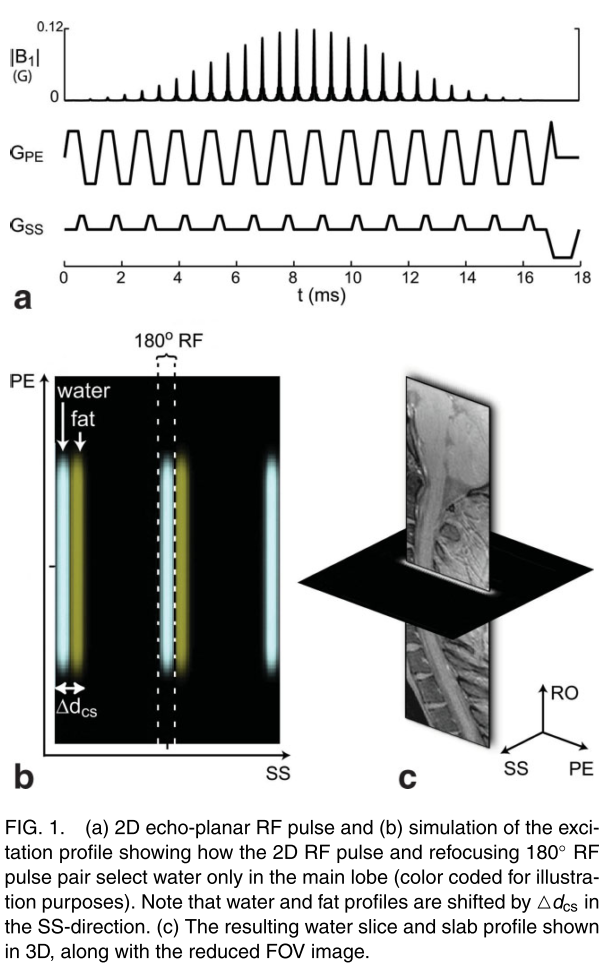
\includegraphics[height=6cm]{SpineDWIfig1}
	\end{column}
\end{columns}
\end{frame}

\subsection{2D Echo-Planar RF Pulse}

\begin{frame}{2D Echo-Planar RF Pulse}
\begin{columns}[T]
	\begin{column}[T]{5cm}
		\begin{itemize}
			\item 2D echo-planar pulses provide control of slice thickness in two orthogonal directions independently by combining two RF pulses
			\item The "slow" (blipped) and the "fast" axes gradients and RF pulses are designed to achieve desired excitation prfiles in each spatial direction
		\end{itemize}
	\end{column}
	\begin{column}[T]{5cm}
		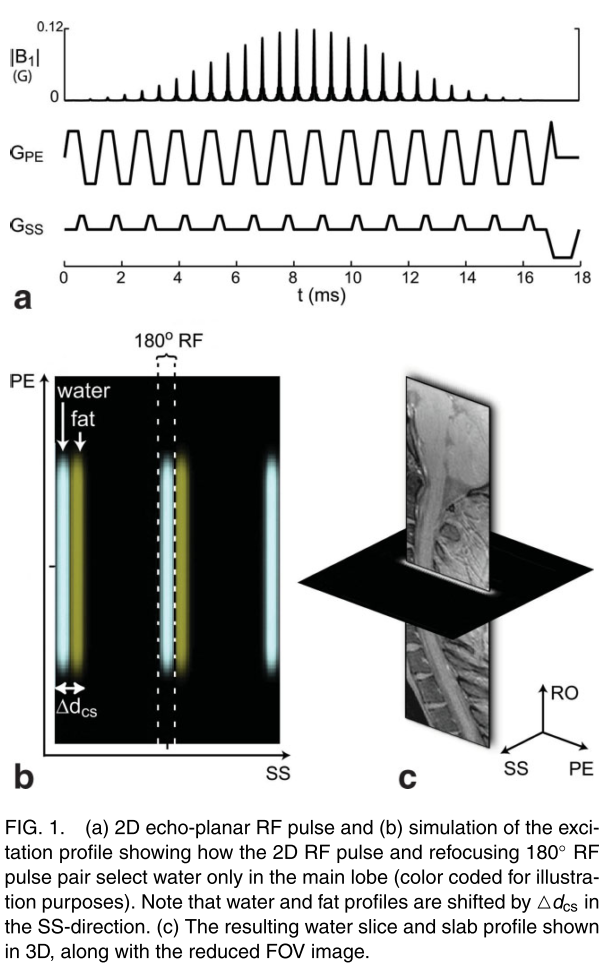
\includegraphics[height=6cm]{SpineDWIfig1}
	\end{column}
\end{columns}
\end{frame}

\begin{frame}{2D Echo-Planar RF Pulse}
\begin{columns}[T]
	\begin{column}[T]{5cm}
		\begin{itemize}
			\item In this paper, the echo-planar RF pulse creates a $90^{\circ}$ flip angle over 4 mm $\times$ 4.5 cm slab
			\item The two orthogonal directions are the slice-select (SS) direction and the slab-select direction (phase encode direction during imaging)
		\end{itemize}
	\end{column}
	\begin{column}[T]{5cm}
		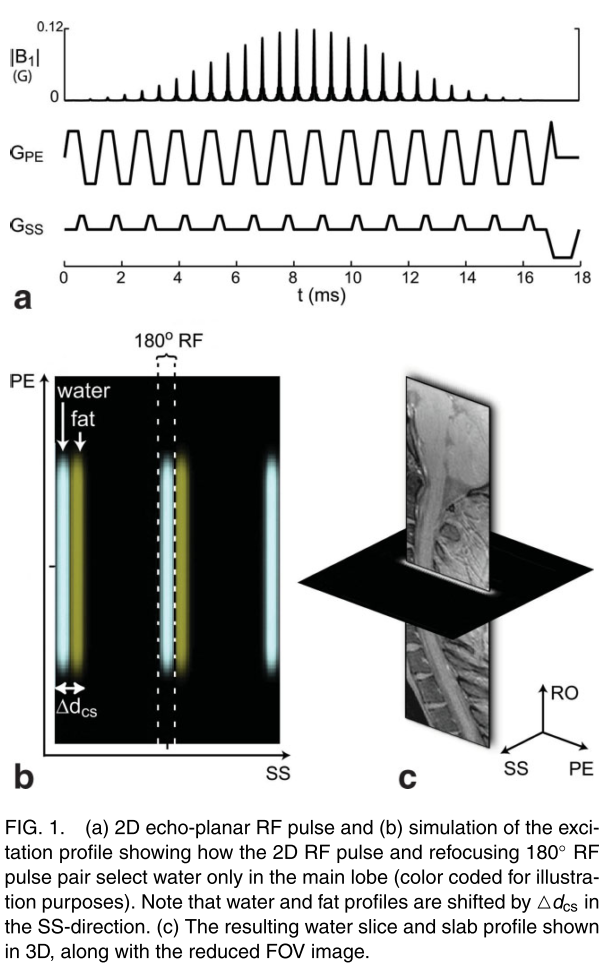
\includegraphics[height=6cm]{SpineDWIfig1}
	\end{column}
\end{columns}
\end{frame}

\begin{frame}{2D Echo-Planar RF Pulse}
\begin{columns}[T]
	\begin{column}[T]{5cm}
		\begin{itemize}
			\item 2D RF pulse reduces PE direction FOV to 4.5 cm, and the pulse duration is 16.8 ms
			\item The excitation profiles for fat and water are displaced in volume along the blipped (SS) direction
		\end{itemize}
	\end{column}
	\begin{column}[T]{5cm}
		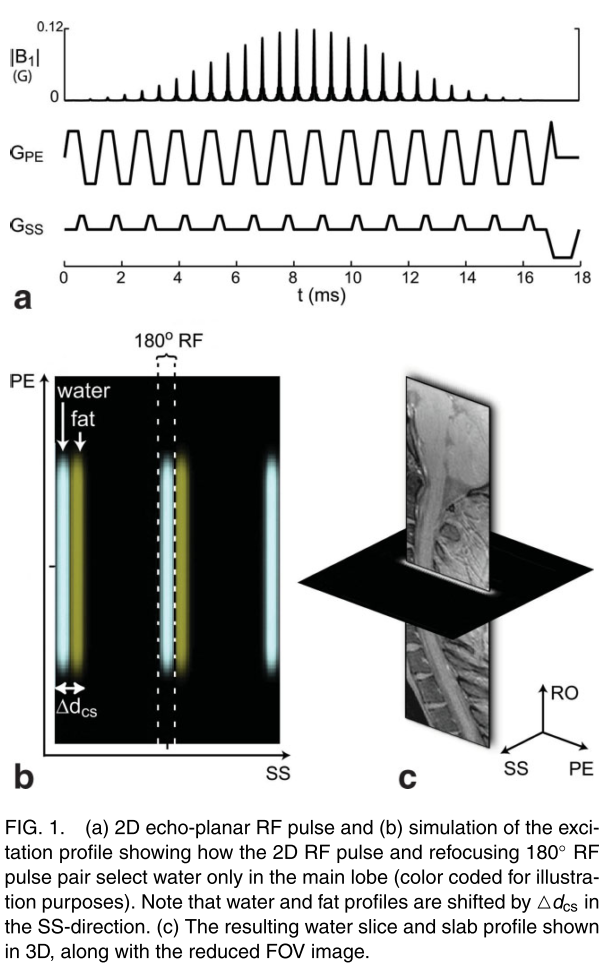
\includegraphics[height=6cm]{SpineDWIfig1}
	\end{column}
\end{columns}
\end{frame}

\begin{frame}{2D Echo-Planar RF Pulse}
\begin{columns}[T]
	\begin{column}[T]{5cm}
		\begin{itemize}
			\item The spatial displacement between fat and water caused by the echo-planar path of the 2D RF excitation pulse is $$\Delta d_{CS}=\frac{N_{blip}f_{CS}T_{fast}}{K_{blip}}$$
			\item The displacement $\Delta d_{CS}$ between fat and water can be designed so that the excited fat profile is entirely outside the water profile
		\end{itemize}
	\end{column}
	\begin{column}[T]{5cm}
		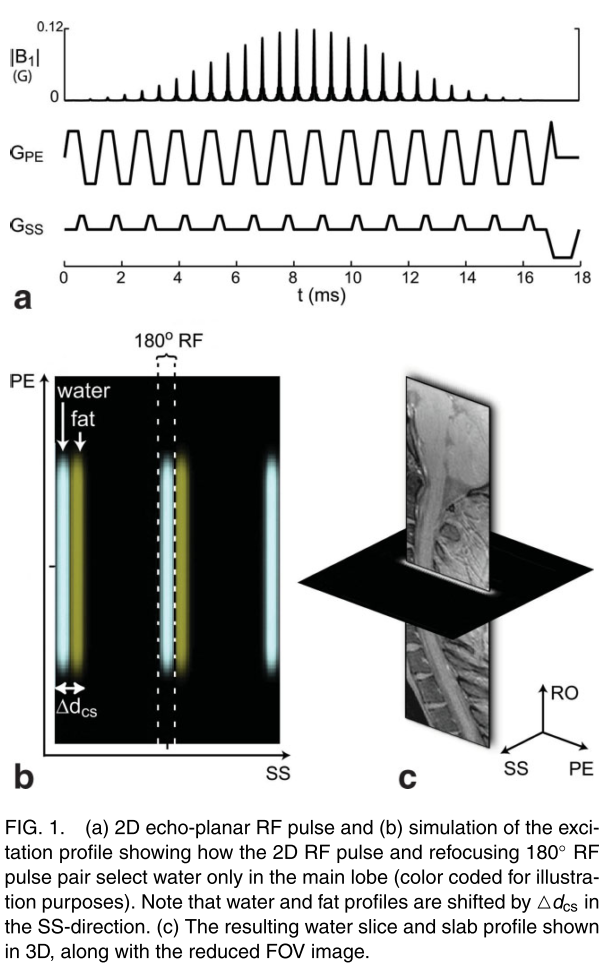
\includegraphics[height=6cm]{SpineDWIfig1}
	\end{column}
\end{columns}
\end{frame}

\begin{frame}{Refocusing RF Pulse}
\begin{itemize}
	\item After 2D RF excitation, a normal $180^{\circ}$ refocusing RF pulse is used, selective in SS direction
	\item Crusher gradients before and after the pulse are used
	\item Using 2D RF excitation pulse and $180^{\circ}$ refocusing RF pulse together suppresses signal outside lobes of periodic 2D excitation and fat signal
\end{itemize}
\end{frame}

\subsection{Multi Slice Imaging}

\begin{frame}{Multi Slice Imaging}
\begin{itemize}
	\item Multi slice imaging is not possible for FOV restriction that uses two separate 1D RF pulses, which excites adjacent slices
	\item 2D echo-planar RF pulses do not excite adjacent slices, making contiguous multi slice imaging possible
	\item Upper limit on number of simultaneously imaged slices: $$max\left(N_{slices}\right)=\frac{\Delta d_{replicate}}{\Delta d_{SS}}=\frac{N_{blip}}{TBW_{SS}}$$
	\item With three sagittal slices the whole pulse sequence takes less than 120 ms per slice, allowing multi slice imaging in one cardiac cycle
\end{itemize}
\end{frame}

%%%%%%%%%%%%%%%%%%%%%%%%%%%%%%%%%%%%%%%%%%%%%%%%%%%%%%%%%%%%%%%%%%%%%%%%%%%
% Methods
%%%%%%%%%%%%%%%%%%%%%%%%%%%%%%%%%%%%%%%%%%%%%%%%%%%%%%%%%%%%%%%%%%%%%%%%%%%
%\section{Methods}
%\subsection{Phantom Experiments}
%\subsection{In Vivo Imaging}
%\subsection{Image Reconstruction}

%%%%%%%%%%%%%%%%%%%%%%%%%%%%%%%%%%%%%%%%%%%%%%%%%%%%%%%%%%%%%%%%%%%%%%%%%%%
% Results
%%%%%%%%%%%%%%%%%%%%%%%%%%%%%%%%%%%%%%%%%%%%%%%%%%%%%%%%%%%%%%%%%%%%%%%%%%%
\section{Results}
\subsection{Phantom Experiment Results}
\subsection{In Vivo Imaging Results}

%%%%%%%%%%%%%%%%%%%%%%%%%%%%%%%%%%%%%%%%%%%%%%%%%%%%%%%%%%%%%%%%%%%%%%%%%%%
% Discussion
%%%%%%%%%%%%%%%%%%%%%%%%%%%%%%%%%%%%%%%%%%%%%%%%%%%%%%%%%%%%%%%%%%%%%%%%%%%
\section{Discussion}

%\begin{frame}{Discussion}
%
%\end{frame}

\subsection{Fat Suppression}
\subsection{Image Reconstruction}

\begin{frame}{Image Reconstruction}
\begin{itemize}
	\item Reduced FOV images with double resolution have quartered SNR
	\item This technique is more robust than multi shot techniques, because no additional navigator echo is needed
\end{itemize}
\end{frame}
\end{document}

